\chapter{Distance of Closest Approach}	\label{dca_appendix}

In Chapter \ref{bosons}, we presented exclusion limits on the gauge coupling of dark bosons at the EIC and MuSIC. These exclusion limits required an estimate of the minimum resolvable displacement of the dark boson, which is related to the transverse distance-of-closest approach (DCA) of the reconstructed trajectories of its final-state decay products. We initially assumed the final states followed straight-line trajectories to estimate the DCA and derive the limits in Section \ref{sec:vector_MuBeD_MuSIC_limits}, then considered the potential effect of a strong magnetic field in Section \ref{sec:displaced_vertex_resolution}. Here, we present derivations of the expressions for the DCA used in those analyses. 

For simplicity, we will focus on the analysis which assumes the final-state leptons experience a transverse magnetic field {\bf B}. The analysis for a straight-line trajectory corresponds to the limit $|{\bf B}| \rightarrow 0$. Given that we assume that all particle trajectories lie in the plane, it is easiest to work in the complex plane.\footnote{I have recently begun learning about geometric algebras, and my feeling is that this derivation would be even cleaner using the conformal geometric algebra. This is left as an exercise for the reader.} We assume that the interaction point lies at the origin, and parametrize the trajectory of the dark boson by
\begin{align}
    {\bf \tilde{d}} &= d e^{i\theta}.
\end{align}
\begin{figure}[t!]
    \centering
    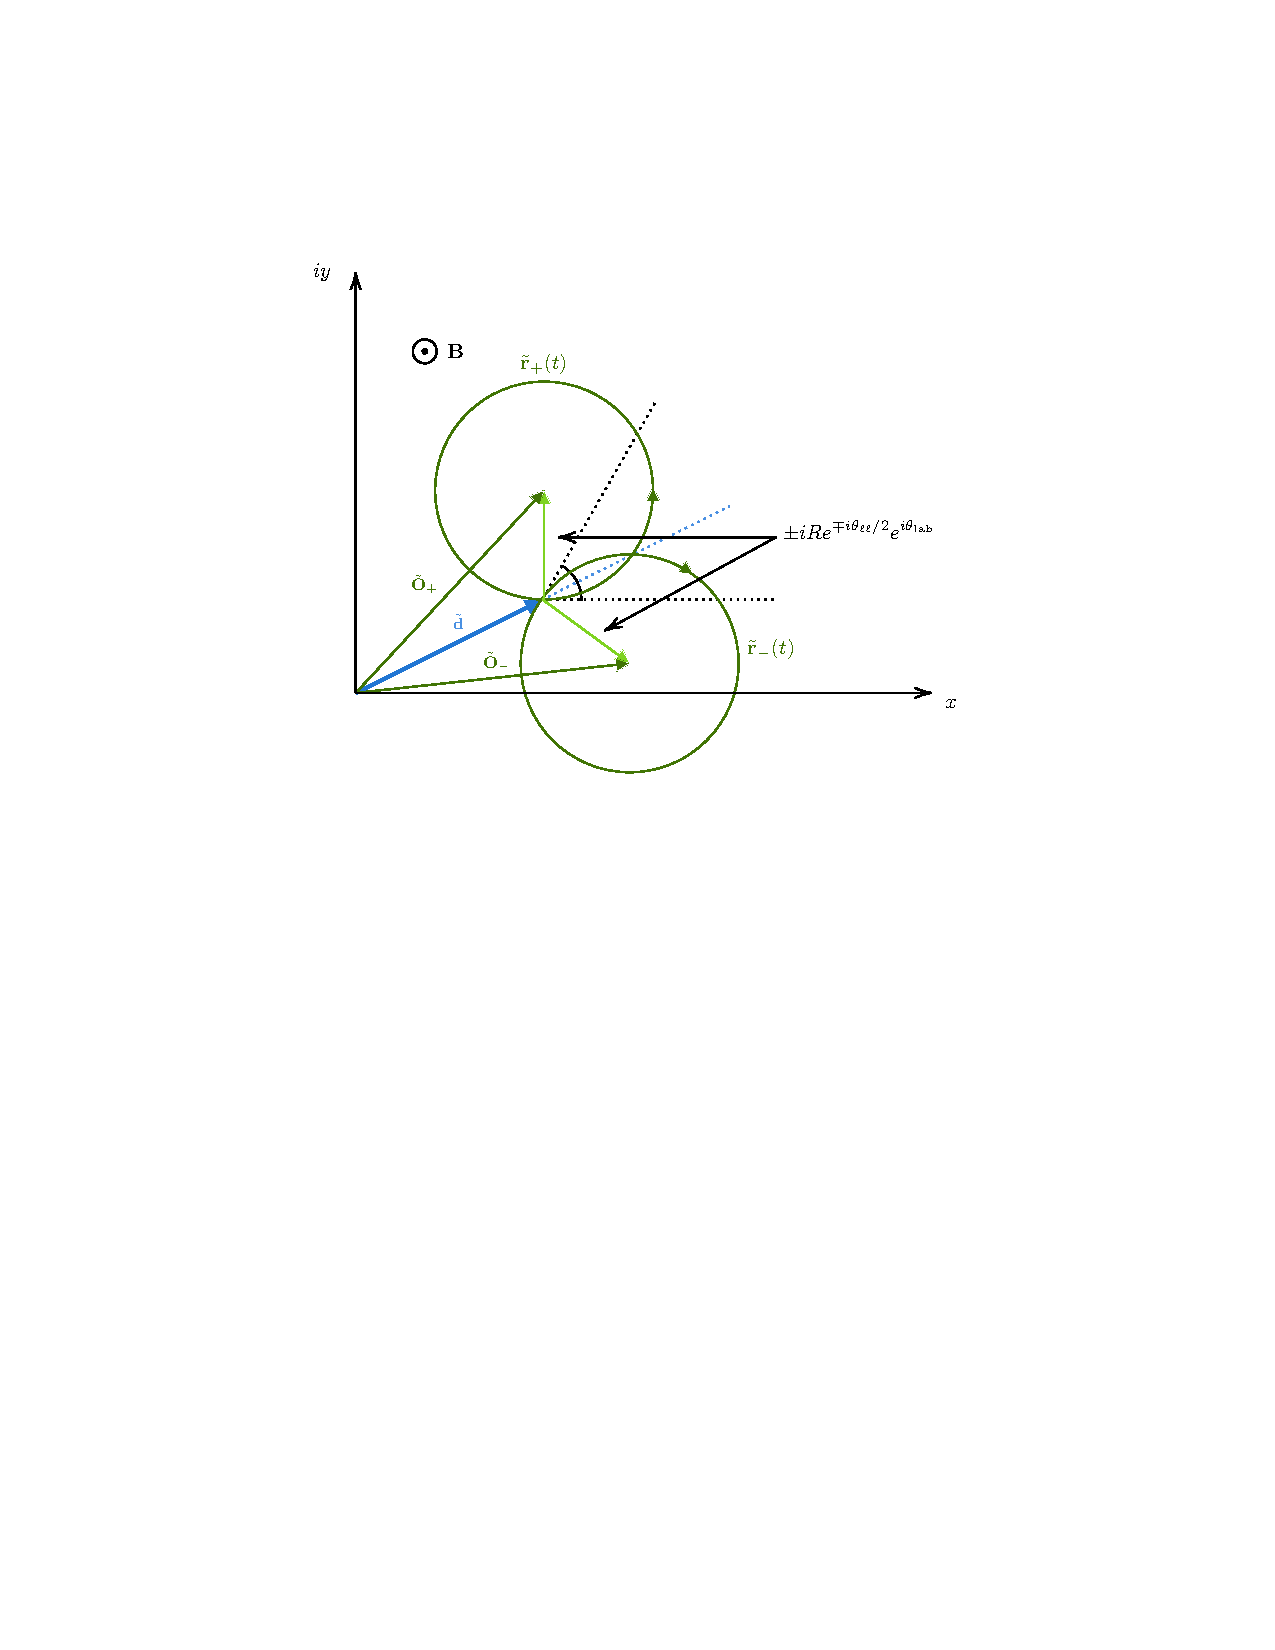
\includegraphics[width=0.8\linewidth]{figures/appendixB/Complex_Geometry.pdf}
    \caption[DCA Analysis Using Complex Geometry]{A schematic representation of the complex geometry used to compute the DCA of the final-state leptons assuming they follow circular arcs.}
    \label{fig:geom_fig}
\end{figure}
If the final-state leptonic decay products of the dark boson open at an angle $\theta_{\ell\ell}$ subject to a magnetic field of magnitude $B = 1\,{\rm T}$, they will follow circular trajectories with radius $R = E_\ell/ecB$. We assume that each lepton carries away half the energy of the dark boson, so $E_\ell = E_{A'}/2$; as such, their angles w.r.t. the direction of the dark boson will each be $\theta_{\ell\ell}/2$. Without loss of generality, we can assume that the magnetic field points out of the page, and that the $\ell^-$ is emitted {\it counterclockwise} relative to the $\ell^+$. A schematic of our set-up is shown in Fig.~\ref{fig:geom_fig}. The alternate orientation (the $\ell^-$ emitted clockwise relative to the $\ell^+$) is encapsulated by taking $R \rightarrow -R$. With these assumptions, the location of the center of the trajectories of the $\ell^\pm$ is given by
\begin{align}
    \tilde{\bf O}_{\pm} &= (d \pm i R e^{\mp i\theta_{\ell\ell}/2})e^{i\theta}\nonumber \\
                        &= \tilde{\bf d} \pm i R e^{i\theta \mp i \theta_{\ell\ell}/2}
\end{align}
and their trajectories are parametrized by
\begin{align}
    \tilde{\bf r}_\pm(t) &= \tilde{\bf O}_{\pm} \mp iR e^{i\theta \mp i\theta_{\ell\ell}/2}e^{\pm it}\nonumber\\
        &= \tilde{\bf d} \pm iR(1-e^{\pm it})e^{i\theta \mp i\theta_{\ell\ell}/2}\nonumber\\
        &= \tilde{\bf d} + 2R\sin{(t/2)}e^{i\theta \mp i{\theta_{\ell\ell}/2} \pm it/2}
\end{align}
where we have chosen $t$ such that $t > 0$ corresponds to the trajectories {\it after} decay of the dark boson, and $t < 0$ corresponds to the reconstructed trajectories.\footnote{For $R < 0$, one must replace $t$ with $-t$ to retain this property.} The DCA of each trajectory to the interaction point is given by
\begin{align}
    {\rm DCA}_{\pm} &= \min_{t}{\left|\tilde{\bf r}_{\pm}(t)\right|}.
\end{align}
The distance from either trajectory to the interaction point can be written
\begin{align}
    \left|\tilde{\bf r}_{\pm}(t)\right|^2 &= |\tilde{\bf d}|^2 + 4R^2\sin^2{(t/2)} + 4{\rm Re}\left\{\tilde{\bf d}^* R \sin{(t/2)}e^{i\theta \mp i{\theta_{\ell\ell}/2} \pm it/2}\right\}\nonumber\\
    &= d^2 + 4R^2\sin^2{(t/2)} + 4dR\sin{(t/2)}\cos{((t - \theta_{\ell\ell})/2)} \nonumber\\
    &= d^2 + 2R^2(1-\cos{t}) + 2dR\left[\sin\left(t-\theta_{\ell\ell}/2\right)+ \sin{(\theta_{\ell\ell}/2)}\right].\label{eq:dist}
\end{align}
Notably, dependence on $\ell^\pm$ has dropped out. In particular, the circular trajectories in Fig.~\ref{fig:geom_fig} are equidistant from the origin (interaction point), and we have chosen a parametrization such that this is manifest in Eq.~\ref{eq:dist}. Those values of $t$ which extremize the distance are then given by
\begin{align}
    2R^2\sin{t} + 2dR\cos{(t - \theta_{\ell\ell}/2)} &= 0
\end{align}
which has solutions
\begin{align}
    t &= \pm \arccos\left(\pm \frac{R+d\sin{(\theta_{\ell\ell}/2)}}{\sqrt{d^2 + R^2 + 2dR\sin{(\theta_{\ell\ell}/2)} }}\right)
\end{align}
where the signs no longer correspond to $\ell^\pm$ labels, and any combination of the signs is a valid solution. Through explicit evaluation, we find that the value of $t$ depends on whether $R > 0$ or $R < 0$ (which corresponds to swapping the $\ell^+$ and $\ell^-$ in the final-state). We have
\begin{align}
    t_> &= -\arccos\left(\frac{R + d\sin{(\theta_{\ell\ell}/2)}}{\sqrt{d^2+R^2}}\right)\\
    t_< &= \arccos\left(\frac{|R| - d\sin{(\theta_{\ell\ell}/2)}}{\sqrt{d^2+|R|^2}}\right)
\end{align}
which, when substituted into our expression for $|\tilde{\bf r}_{\pm}(t)|^2$, yield
\begin{align}
    ({\rm DCA}_>)^2 &= \left|\sqrt{R^2 + d^2 + 2dR\sin{(\theta_{\ell\ell}/2)}} - R\right|^2
\intertext{and}
    ({\rm DCA}_<)^2 &= \left|\sqrt{|R|^2 + d^2 - 2d|R|\sin{(\theta_{\ell\ell}/2)}} - |R|\right|^2.
\end{align}
For each of these scenarios, we define the {\it average transverse DCA}, $\overline{{\rm DCA}_{\rm 2D}}$, as the average of the transverse components of the DCA for each lepton. Notably, the DCA is the same for both of them, but the transverse components are given by
\begin{align}
    {\rm DCA}_{\rm 2D}^{\pm} &= {\rm DCA}\cos{(\theta \pm \theta_{\ell\ell}/2)}
\end{align}
yielding an average
\begin{align}
    \overline{{\rm DCA}_{\rm 2D}} &= \frac{1}{2}\left({\rm DCA}_{\rm 2D}^+ + {\rm DCA}_{\rm 2D}^{-}\right) \nonumber\\
    &= {\rm DCA}\cos{\theta}\cos{(\theta_{\ell\ell}/2)}.
\end{align}
Hence, given a minimum DCA resolution ${\rm DCA}_{\rm 2D}^{\rm min}$ (and defining ${\rm DCA}^{\rm min} \equiv {\rm DCA}_{\rm 2D}^{\rm min}/(\cos{\theta}\cos{(\theta_{\ell\ell}/2)})$ for convenience), the minimum resolvable displacement $d^{\rm min}$ can be found by solving the equation
\begin{align}
    \left|\sqrt{R^2 + d^2 + 2dR\sin{(\theta_{\ell\ell}/2)}} - R\right| > {\rm DCA}^{\rm min}
\end{align}
for $R > 0$ and
\begin{align}
    \left|\sqrt{|R|^2 + d^2 - 2d|R|\sin{(\theta_{\ell\ell}/2)}} - |R|\right| > {\rm DCA}^{\rm min}
\end{align}
for $R < 0$. The first equation is slightly easier to solve, because the term inside of the absolute value is always positive. In contrast, the sign of the absolute value in the second equation is conditional on the relative size of $|R|\sin{(\theta_{\ell\ell}/2)}$ and $d$. After evaluation of all possible solutions, we find
\begin{align}
    d_{>}^{\rm min} &= -R\sin{(\theta_{\ell\ell/2})} + \begin{cases}
    \sqrt{({\rm DCA}^{\rm min})^2 - 2R({\rm DCA}^{\rm min})+R^2\sin^2{(\theta_{\ell\ell}/2)}}\\
    \sqrt{({\rm DCA}^{\rm min})^2 + 2R({\rm DCA}^{\rm min})+R^2\sin^2{(\theta_{\ell\ell}/2)}}
    \end{cases}
\end{align}
and
\begin{align}
    d_{<}^{\rm min} &= |R|\sin{(\theta_{\ell\ell}/2)} + \begin{cases}
    -\sqrt{({\rm DCA}^{\rm min})^2 - 2|R|({\rm DCA}^{\rm min})+|R|^2\sin^2{(\theta_{\ell\ell}/2)}}\\
    \sqrt{({\rm DCA}^{\rm min})^2 + 2|R|({\rm DCA}^{\rm min})+|R|^2\sin^2{(\theta_{\ell\ell}/2)}}
    \end{cases}
\end{align}
where the upper cases are chosen unless the resulting expression is negative or complex. To complete our analysis, we assume that half of the dark bosons decay with the $\ell^-$ counterclockwise relative to the $\ell^+$ (the `$<$' orientation) and half of the dark bosons decay with the $\ell^-$ clockwise relative to the $\ell^+$ (the `$>$' orientation).

In the limit of infinite $R$, we can recover the straight-line trajectories. We find 
\begin{align}
    d_{\rm min} \equiv \lim_{R \rightarrow \infty}{ d}^{\rm min}_> = \lim_{|R| \rightarrow \infty}{d}^{\rm min}_< = \frac{\rm DCA^{\rm min}_{\rm 2D}}{\sin{(\theta_{\ell\ell}/2)}}.
\end{align}
Finally, we must provide an estimate for the opening angle $\theta_{\ell\ell}$. We can approximate $\theta_{\ell\ell}$ using four-momentum conservation:
\begin{align}
    \gamma m_{A'} &= 2\gamma_\ell m_\ell\\
    \gamma v m_{A'} &= 2\gamma_\ell v_\ell m_\ell \cos{(\theta_{\ell\ell}/2})
\end{align}
which gives
\begin{align}
    \sin{\theta_{\ell\ell}} &= \frac{2\gamma v m_{A'}}{\gamma^2 m_{A'}^2 - 4m_\ell^2 }\sqrt{m_{A'}^2 - 4m_{\ell}^2} \label{eq:exact}\\
    &\approx \frac{2v}{\gamma}.
\end{align}
Hence, we take $\theta_{\ell\ell}\approx 2v/\gamma$ for our analyses. Use of the exact formula (\ref{eq:exact}) will yield a better estimate of the limits near mass threshold ($m_{A'} \gtrsim 2m_\ell$), but should otherwise have a negligible effect on the results.